\documentclass[10pt]{article}
\usepackage[utf8]{inputenc}
\usepackage{url}
\usepackage{hyperref}
\usepackage{amsmath}
\usepackage{amsfonts}
\usepackage{amssymb}
\usepackage{graphicx}
\usepackage{float}
\usepackage{lipsum}
\usepackage{multicol}
\usepackage[table]{xcolor}
\usepackage[square, numbers]{natbib}
\usepackage[font=small]{caption}
\addtolength{\abovecaptionskip}{-3mm}
\addtolength{\textfloatsep}{-5mm}
\setlength\columnsep{20pt}

\usepackage[a4paper,left=1.50cm, right=1.50cm, top=1.50cm, bottom=1.50cm]{geometry}


\author{}

\title{2022 Fetch Rewards Machine Learning Engineering Apprenticeship}

\begin{document}
	
	\begin{center}
		{\Large \textbf{Minimage: An Image Compression Web App}}\\[1ex]
		{\large{2022 Fetch Rewards Machine Learning Engineering Apprenticeship}}\\
		\vspace{1em}
		{\large Will Foote}\\
		\vspace{.75em}
		\textit{Statistics, Public Affairs at UCLA (June 2022)}
		
\begin{figure}[H]
    \centering
	
\includegraphics[width=.5\columnwidth]{home.png}
	\caption{The minimage home page.}
	\label{fig:fig1}
\end{figure}

	\end{center}
	

	%\begin{center}
	%	\rule{150mm}{0.2mm}
	%\end{center}		

	%\begin{abstract}
	
	%This document contains the instructions for preparing a valid 2022--2023 Bloomberg Data Science Ph.D./Postdoc Fellowship Application research proposal. This document conforms to its own specifications and is an example of what your proposal should look like.
	
	%The abstract should briefly describe the proposal and make the case for the proposal to non-experts in your particular field. The rest of the proposal should be directed at a technical data science audience.
	
	%\textbf{Collaborators}: list the names and affiliations of expected collaborators on the project here
	%\end{abstract}

	%\begin{center}
	%	\rule{150mm}{0.2mm}
	%\end{center}		

	\vspace{3mm}
	
\begin{multicols*}{2}

\section{Introduction}
 
It was not enough to just create a function that plots evenly spaced points/pixels on a rectangle and app-ify it. As with most things, I wanted to do more. So, I brainstormed ways to make such a program, but also how that program might be used -- as a part of a larger, more scalable goal. But I also wanted to tell a story: one not written by words or directed cinematically, but one that was subtle and relied on cohesive themes/a personal brand that could catalyze a seamless user experience.

To achieve these two goals I landed on creating a ``proof of concept" version of an image compression app which uses Principal Components Analysis (an unsupervised machine learning technique) to reduce the size of the picture at minimal cost of quality and then renders the compressed image using the original pixel-plotting program.

Obviously, this isn't production-ready nor do I necessarily believe it's a viable solution (to a problem that doesn't really need to be solved -- image compression is easy already), but I'll outline these limitations later on. As such, take the verbosity and written flamboyance on the website with a grain of salt. Few of them are my actual beliefs but rather those of a hypothetical, overconfident CEO of this random company. 

In total, I hope this project illustrates my ability to tell stories through products that make sense and are easily accessible for frontend users and backend collaborators alike. Also, I suppose, that my coding practices and data science knowledge are at least decent. \vspace{-2ex}

\section{Frameworks Used}

\subsection{App Development: Flask}

I used the Flask framework to build the app. It's initalized with app.py and $\_\_$init$\_\_$.py and the different "views" for different webpages are in application/routes.

\subsection{Python Libraries: Matplotlib, Numpy, Pandas, Sklearn, Plotly, WTForms}

To answer the pixel-plotting question, I only used Numpy and base Python for manipulating and creating different data structures (e.g. lists and arrays). To analyze the data with PCA I used Sklearn to scale and mine the data of an image to test the program on called ``lena.raw.''

On the user side of things, I used WTForms to easily interact with POST requests made by a user on the website and Matplotlib/Plotly to render the compressed image or visualize the pixel-plotting itself (i.e. answer the question), respectively. I used Plotly for the interactivity of the graph and it's ease-of-integration with flask. I realized that this interactivity could be a barrier to scalability. For example, a 512x512 image is already 262,144 points to graph. I don't think Matplotlib is too quick of an alternative but its non-interactive nature made it quicker and less computationally expensive (from my experience testing both).

\subsection{Styling: Bootstrap}

For the HTML and CSS, I used some jinja to display Python variables as text on the webpage. For most styling things, I relied on Bootstrap to make things pretty given limited time to dive into creating a unified CSS theme.

\subsection{Containerization: Docker}

For those who haven't heard of Docker, essentially a Docker container allows a user who may have different computer settings/architecture than mine run the app via an "image" of my system in a "contained" environment (hence the terms Docker image and Docker container). 

I built the image of the application using Docker's command line interface (CLI). Somewhat noteworthy is that that I've been working on an M1 Macbook, so I made sure to build a multi-architecture image that compatible with linux/amd64 and linux/arm64 operating systems. 

\subsection{Hosting: Docker Hub/Github}

While the raw files are posted on my Github repository, I created a Docker Hub repository for storing the images themselves.

\section{How To Run The App}

Getting the app running locally is a matter of pulling the Docker Image from Docker Hub and running it inside a container. The code below should get you through that process easily. Recall again that I'm using MacOS, so \underline{\href{https://docs.docker.com/engine/reference/commandline/cli/}{here's}} the docker command line documentation for getting started.

\subsection{General Steps}

\begin{enumerate}
\item Check if docker is Running
\item Run docker if not
\item Pull minimage the Docker image from Docker Hub
\item Run the image in a container
\item Launch the website
\end{enumerate}

\subsection{Code}

\begin{enumerate}
\item service docker status
\item service docker start \#(if docker is not running)
\item docker pull williamfoote/minimage:latest-multiarch
\item docker run -dp 8000:5000 minimage:latest-multiarch
\item http://localhost:8000/
\end{enumerate}

Note: -dp in step four corresponds to running the container in the background (i.e. "detached" mode) and p maps the host's port 5000 to the container's port 3000.

Note: You need to navigate to the listed address, \underline{\textbf{which will be different}} from the one located in the Flask logs. This has to do with the two separate network namespaces we're working in. Indeed, the app is listening on the pictured address -- within the \textit{container's} namespace. But your browser is located on your main namespace which is a completely different 127.0.0.1:5000. The name's are the same, the results are not. \textbf{Go to http://localhost:8000/ instead.}

\begin{figure}[H]
    \centering
	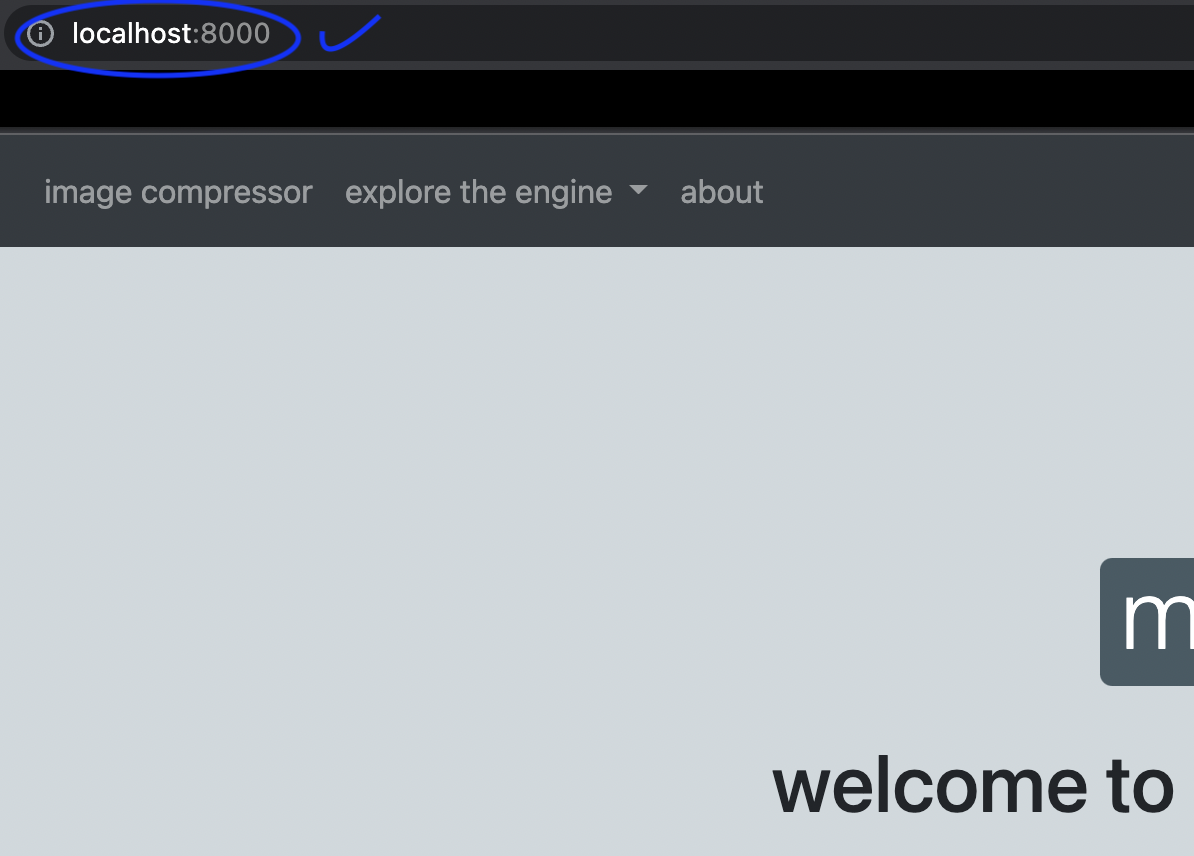
\includegraphics[width=\columnwidth]{right.png}
	\caption{Correct address to go to in step 5.}
	\label{fig:fig2}
\end{figure}

\begin{figure}[H]
    \centering
	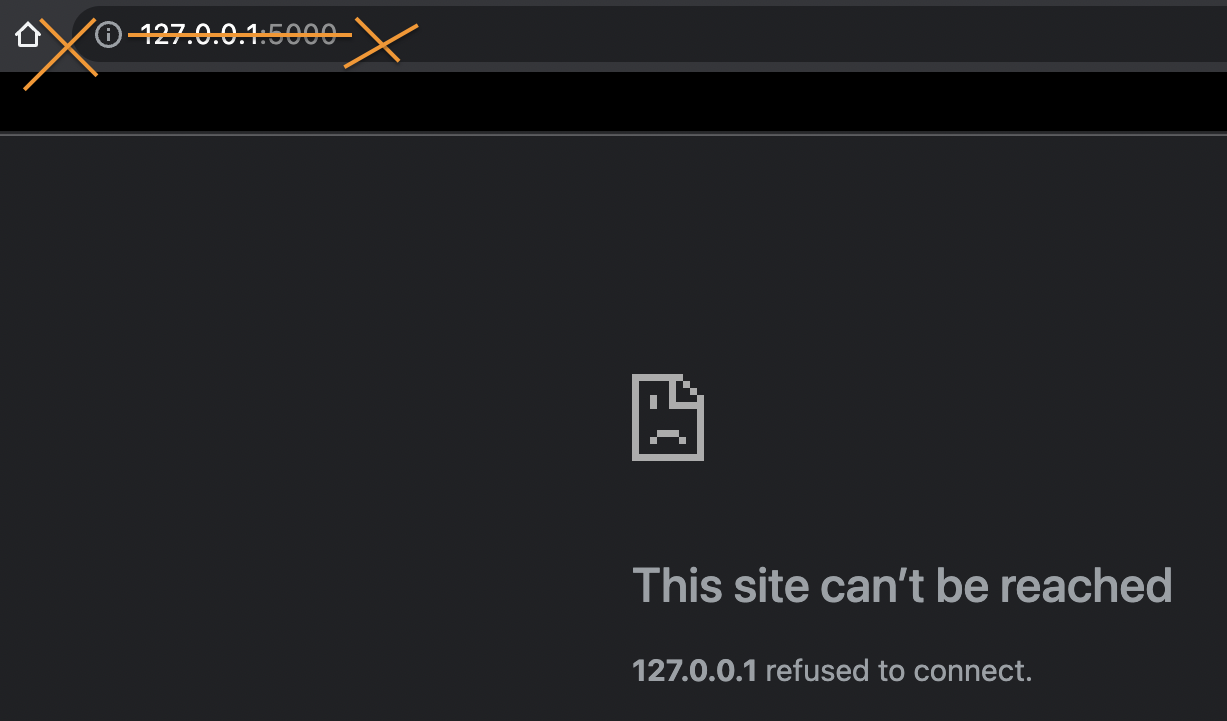
\includegraphics[width=\columnwidth]{wrong.png}
	\caption{\textbf{Incorrect} address to go to in step 5.}
	\label{fig:fig3}
\end{figure}

\section{An App Tutorial}

\subsection{``explore the engine"}

\begin{figure}[H]
    \centering
	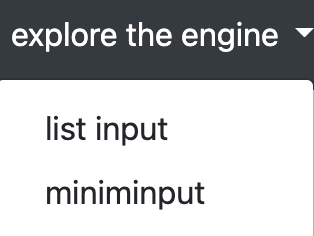
\includegraphics[width=.5\columnwidth]{ete.png}
	\caption{There are two options for running the pixel plotter.}
	\label{fig:fig4}
\end{figure}
 
To run the program that is requested for this assignment, check out the two "explore the engine" pages. There are two options "list input" and "miniminput." Note, the results of each page should be the same, the process to get there is just different.

\subsection{``explore the engine: list input"}

I included the list input in the app to fulfill the requirements. On this page, a user can paste a list of corner points and a tuple of the shape of the desired grid, with the option to graph the results using Plotly and how many decimal places to round to. 

The page displays the solutions list corresponding to the "mxnx2 where m is the number of rows in the input image and n is the number of columns in the input image" (per the assignment instructions). If the user elects to visualize the results, the graph of the resulting grid is chosen. Note, depending on the rounding choices, the points may be unevenly distributed.

\subsubsection{``list input's'' Limitations}

But, I felt that it wasn't the most accessible for a production-level app for two reason. For one, there are potential security issues with the implementation of my app, which uses ast.literal\_eval to take in the character-strings that the list and tuple are returned as and turns them into their Python versions. While the \href{https://stackoverflow.com/questions/4710247/python-3-are-there-any-known-security-holes-in-ast-literal-evalnode-or-string#:~:text=The\%20documentation\%20states\%20it\%20is,if\%20it\%20is\%20a\%20literal.}{consensus} seemed to be that it's safe, it doesn't totally sit right with me as a lasting solution. And, I'm also realizing now that there are probably other JSON-utilizing methods that can parse the data better. I'm open to suggestions on this end!

\subsection{``explore the engine: miniminput"}

On the other hand, and more importantly, I didn't feel like this solution was cohesive with the accessible brand I was trying to create for the app. So, I created a more user-friendly version where the corner points and shape are taken is an integer inputs in the form. Knowing Python and its data structures shouldn't be a barrier to my app! 

\subsection{``image compressor"}

\begin{figure}[H]
    \centering
	
\includegraphics[width=.5\columnwidth]{ic.png}
	\caption{The compressor itself is on its own page.}
	\label{fig:fig5}
\end{figure}

This pages is a proof of concept of how I might approach the problem of image compression using my plotting function (called imagePixels) and the unsupervised machine learning technique called Principal Components Analysis.

\subsubsection{Under the Hood: Principal Components Analysis}

PCA is a type of technique called ``dimensionality reduction" that aims to turn "p" variables of a dataset into "k" (where k < p) variables called ``principal components'' that hopefully explain just as much of the underlying trends and structure of the data as before. 

As it pertains to images, if we have a 512x512 image you could say the data has 512 variables (i.e. columns). PCA would try to reduce the need for 512x512 = 262,144 unique pixels into a smaller number of variables by throwing out the highly correlated ones. One way to think of it is that if a set of pixels are in close proximity and very similar to each other, we probably don't need all of those unique pixels to be stored in the file to get the gist of the picture. Hence, after applying PCA, the image should be less bytes of data. 

Lots of \underline{\href{https://towardsdatascience.com/image-compression-using-principal-component-analysis-pca-253f26740a9f}{research}} has been written about Principal Components Analysis and image compression so this is an implementation that builds off of those ideas. 

\subsubsection{Running the compressor}

Right now, there's only one image that the program works on called "Lena," which is a famous picture in the image processing field and is tied to the roots of the creation of the JPEG file format. I used it because it's in RAW format, so 512 x 512 pixels are actually in the data (whereas when I tried with PNG's and JPEG's, there were far fewer pixels -- which makes sense that their smaller file sizes compared to RAW correspond to how many data/pixel is stored in them).

Anyways, a user selects the dimensions of the photo (locked into 512x512 for this test case), the picture to analyze (also locked to one option) as well as how much of the original quality to keep in a percent. 

    \begin{figure}[H]
        \centering
    	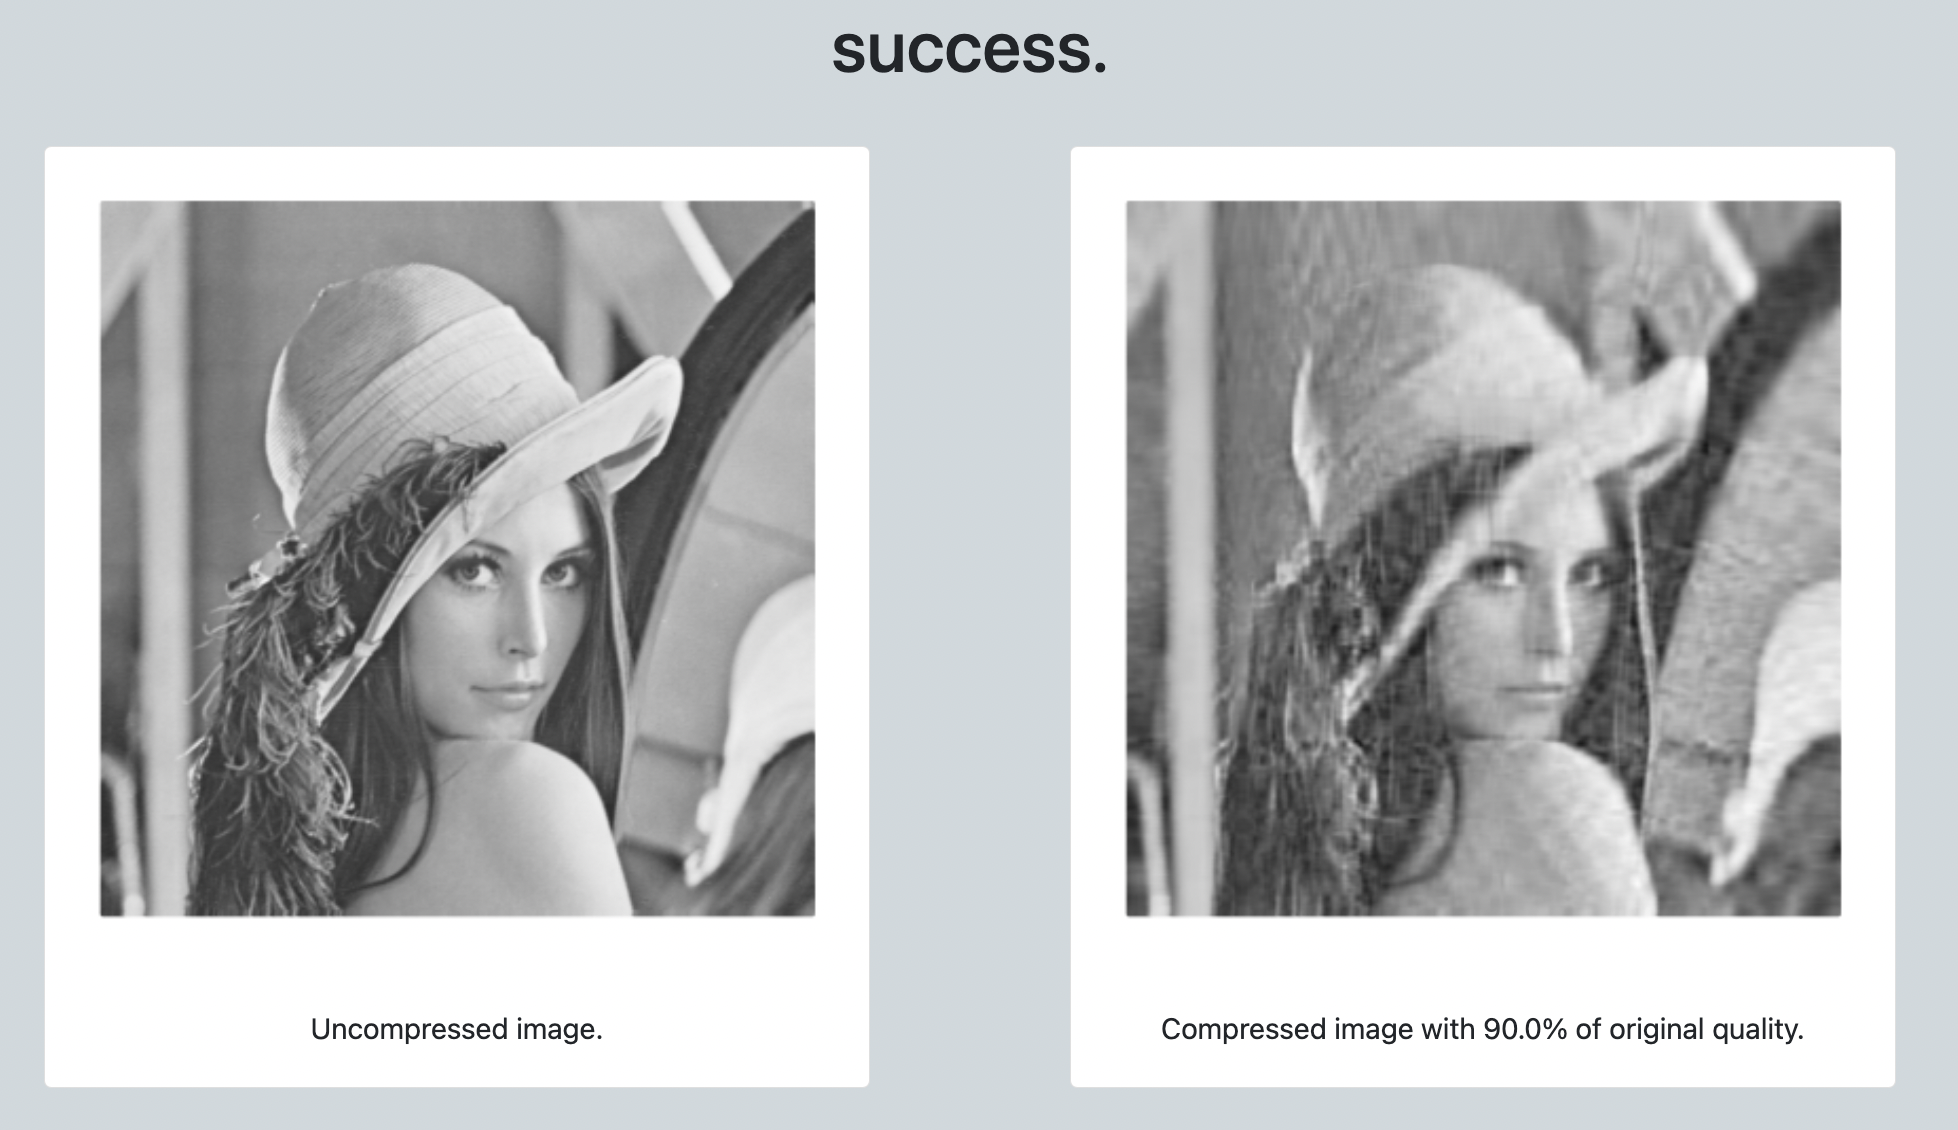
\includegraphics[width=\columnwidth]{compressed.png}
    	\caption{The results are promising at the 90\% threshhold.}
    	\label{fig:fig6}
    \end{figure}

The results are plotted side by side after the form is submit and the analysis is ran. This is the slowest functionality on the app because a lot needs to be done. I think the main bottleneck is the rendering-via-graphing points, if I had to guess. 

Nonethelss, the results are actually sort of promising. In a very statistically-unsound way, I downloaded the 75\%-quality version (I ran the algorithm to get a 100\% quality version of the picture and stored it in the static files so it doesn't need to be rendered every time) and it was 70 kb to the original's 116 kb (this is lower than expected as 75\% of 116 is 87 kb!). Not terrible!

This discrepancy makes sense with the power of PCA in mind, though. As the graph below shows, we can keep almost 100\% of the picture quality with only the 100 most important ``principal components" (i.e. recall these are the essentially the 100-most highly coordinated variables of the 512 total in the 512x512 image). 

\begin{figure}[H]
    \centering
	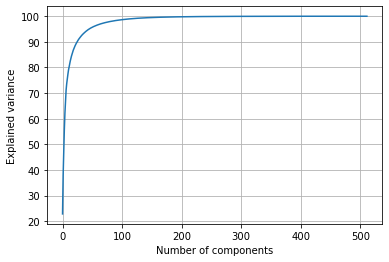
\includegraphics[width=.75\columnwidth]{pca.png}
	\caption{A graph of the amount of variation explained (i.e. remaining image quality \%) versus the amount of pixels we elect to keep.}
	\label{fig:fig6}
\end{figure}

In other words, we get about 99\% image quality with 100/500 = 1/5 of the original dataset. In fact, 70 kb isn't even small enough! It should be much lower based on this graph and explanation. I imagine this has to do with how the graphs are exported and stored as .png's, but that's a little beyond my pay-grade at the moment.



\subsubsection{``image compressor's'' Limitations}

Note, this is far from a production-ready implementation. For one, plotting the pixels one by one using Python's MatPlotLib or Plotly graphing libraries is probably not the most efficient. I highly doubt they are able to quickly plot 262,000+ points on a scalable level. At least there are probably better alternatives. Moreover, the app only works on greyscale photos at the moment, mostly due to limitations on the problem to not use image processing libraries. With more time I think I could implement an RGB version of this program with numpy/pandas as the main and only external libraries, but image processing libraries like Pillow (PIL) and OpenCV would definitely make this more manageable.

\section{A Surface Level Coding Walkthrough}

I'll go over the general use of the four main classes I created for this project which aimed to achieve four main functionalities. These included classes imagePixels, graphItMPL, graphItPlotly, and cornersFromEasy. imagePixels gets the solution to the assignment's problem. graphitMPL and graphItPlotly take in an imagePixels object and dimensions of the desired plot and output a matplotlib or plotly plot, respectively. cornersFromEasy is the lightest-weight of the four and simply takes the input from the ``miniminput" form and returns the corner points as a list for use with imagePixels.

\subsection{imagePixels}

imagePixels functions by unpacking the input, creating the desired x, y points, and then packaging the results in the requested format. The idea behind this process is that if I unpack the list of x, y coordinates into their x and y components respectively, I can find the minimum x, minimum y, maximum x, and maximum y values. This information is enough to get the grid of points across the rectangle using numpy. That is, if we have the minimum values of each coordinate and how many dots we are supposed to have along each coordinate axis, we just have to make all the permutations of these pairs. I used np.linspace and list comprehension for these two tasks, respectively.

Note, I chose list comprehension over a regular for loop because I found that it was faster (using the timeit library). One other method that could be worth looking into is the itertools package which is known for doing similar tasks to the goals I had. Nonetheless, I wanted to stay within the base ecosystem and use numpy to achieve the answer.

\subsection{graphItMPL}

The two graphIt classes are pretty much inheritances of the imagePixels class (even though I didn't code them that way for some reason). In essence, they define methods to apply to the imagePixels class. They both take in the dimension (2D for all the examples on the app right now) and the imagePixels object. Note, dimension is set because I want to be able to take higher dimensions at some point and get similar outputs for those spaces. And, despite the same input, the two functions have slightly different outputs. 

graphItMPL saves the file as a temporary png which can be implemented in the HTML of the site as an image. 

\subsection{graphItPlotly}

On the other hand, graphItPlotly returns the figure itself as a JSON object. This allows the website to host the graph as an interactive plot. It's also why it wasn't a viable solution for rendering in the imageCompressor stage. I imagine that Plotly is interactive because it is vectorized. That is, the picture we see that is rendered is represented by vectors which is a quantity with magnitude and direction. This allows users to zoom in very far without losing quality (whereas zooming in on a matplotlib graph would be pixelated quickly.

But, the tradeoff is that this becomes incredibly computationally expensive to scale the more pixels there are to graph. If all 262,000 points/vectors of the 512x512 picture have to be moved at once, it makes sense that the program would crash on the average computer.

\subsection{cornersFromEasy}

cornersFromEasy is for use with the ``miniminput" page and simply packages the four numbers the user inputted into an array of the four points. Similar to the logic behind imagePixels itself, if we know the bottom left and top right points on a rectangle, we can also deduce the other two corners by just making the other two permutations of points.

\section{Conclusion}

This was a fun project! Perhaps the most fun one I've done! I hope that in the app that I've created and specifically how I've created it would be a solid foundation for a production-quality one down the road if testers and editors were added to the team. Moving forward, I'd like to think the ideas of this project can be a stepping stone for more research and similar methods in the future. I'm far from the first person to use PCA and image compression together, but it was fun to build off of past people's research and explore with my hands how both of these ideas work together -- and the limitations that such an approach might have.

If you have any questions feel free to email me at \underline{williamfoote1122@gmail.com} or \underline{\href{https://www.linkedin.com/in/william-foote}{connect with me on LinkedIn}}. The full list of project files can be found on \underline{\href{https://github.com/williamfoote/minimage}{the Github repo}} I created for this project and the Docker image details can be found on \underline{\href{https://hub.docker.com/repository/docker/williamfoote/minimage}{the minimage Docker Hub repository}}.

\end{multicols*}
	
\end{document}